%%==========================
%% chapter01.tex for SJTU Master Thesis
%% based on CASthesis
%% modified by wei.jianwen@gmail.com
%% version: 0.3a
%% Encoding: UTF-8
%% last update: Dec 5th, 2010
%%==================================================

%\bibliographystyle{sjtu2} %[此处用于每章都生产参考文献]
\chapter{重复数据检测关键技术}
\label{chap:tech}

\section{全文件检测}
\label{sec:WFD}

WFD(whole file Detection)是以整个文件为查找粒度的检测重复数据方法。首先,对整个文件进行SHA1哈希计算,将这个计算出来的值与现有的已存储下来的值做比较,如果检测到有相同的值,说明这个文件是重复文件,否则,说明这个文件不是重复文件,需要存储下来,并且记下这个文件的SHA1哈希值。

这个方法的优点是非常简单,实现起来非常的容易。但是在实际运用中会暴露很多严重的问题,最典型的就是插入问题和删除问题。两个相同的文件,若在第一个文件开头插入了若干个字节,这个算法将判定这两个文件是完全不相同的文件,这显然是不符合现实的。删除问题也面临着同样的困境,若在第一个文件开头删除了若干个字节,但其它的文件内容保持不变,那么这个算法也将存储两份拷贝。其次,每个文件的大小不同,对于一个系统而言,知道输入文件的规模将大大减小复杂性和提高效率。

\begin{figure}[!hbp]
%\centering
    \begin{minipage}[b]{1\textwidth}
    \captionstyle{\centering}
    \centering
    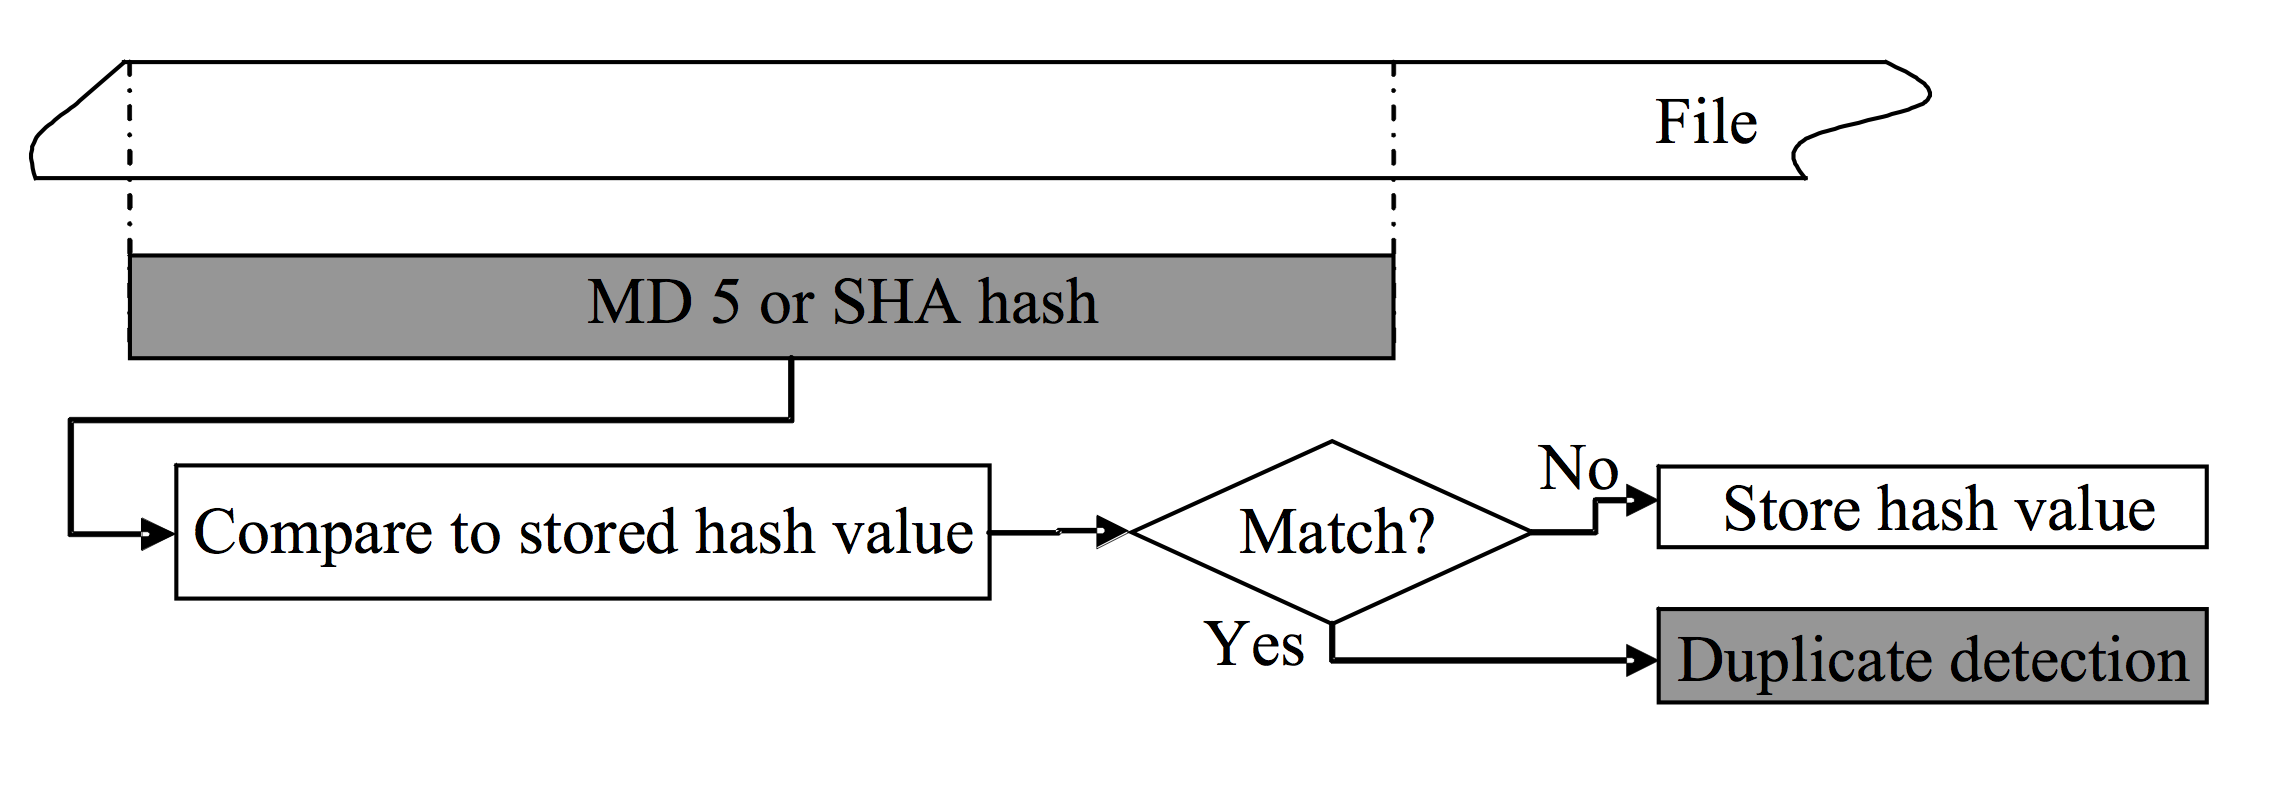
\includegraphics[origin=br,width=15cm]{chap2/wfd.png}
    \bicaption[fig:wfd]{xxx}{WFD技术.}{Fig}{WFD}
    \end{minipage}     
\end{figure}

\section{简单分块}
\label{sec:simpleblock}

图显示的简单分块(Simple blocking)算法把一个文件分成若干不重叠固定大小的分块。计算每一块分块的SHA1哈希值并且把它们存储在一张表中。随着之后的文件划分成分块,它们的SHA1哈希值分别被计算,和已经保存下来的SHA1哈希值做比较,若发现相等,则发现了重复。

这个方法的主要问题是当两个文件只有一个byte不同时,那么将无法检测出重复数据。比如想象这样一种情景,一个文件被复制了,然后在它的开头任意添加了几个bytes的数据。这些添加的字节导致了整个文件块内容的偏移,导致所有分块的边界混乱了。一个相似的例子是当有几个bytes被删除的时候。修改文件的所有分块将不和任意表中的分块相同,所以文件中即使有绝大部分是相同的,但仍然要存储两份拷贝。

\begin{figure}[!hbp]
%\centering
    \begin{minipage}[b]{1\textwidth}
    \captionstyle{\centering}
    \centering
    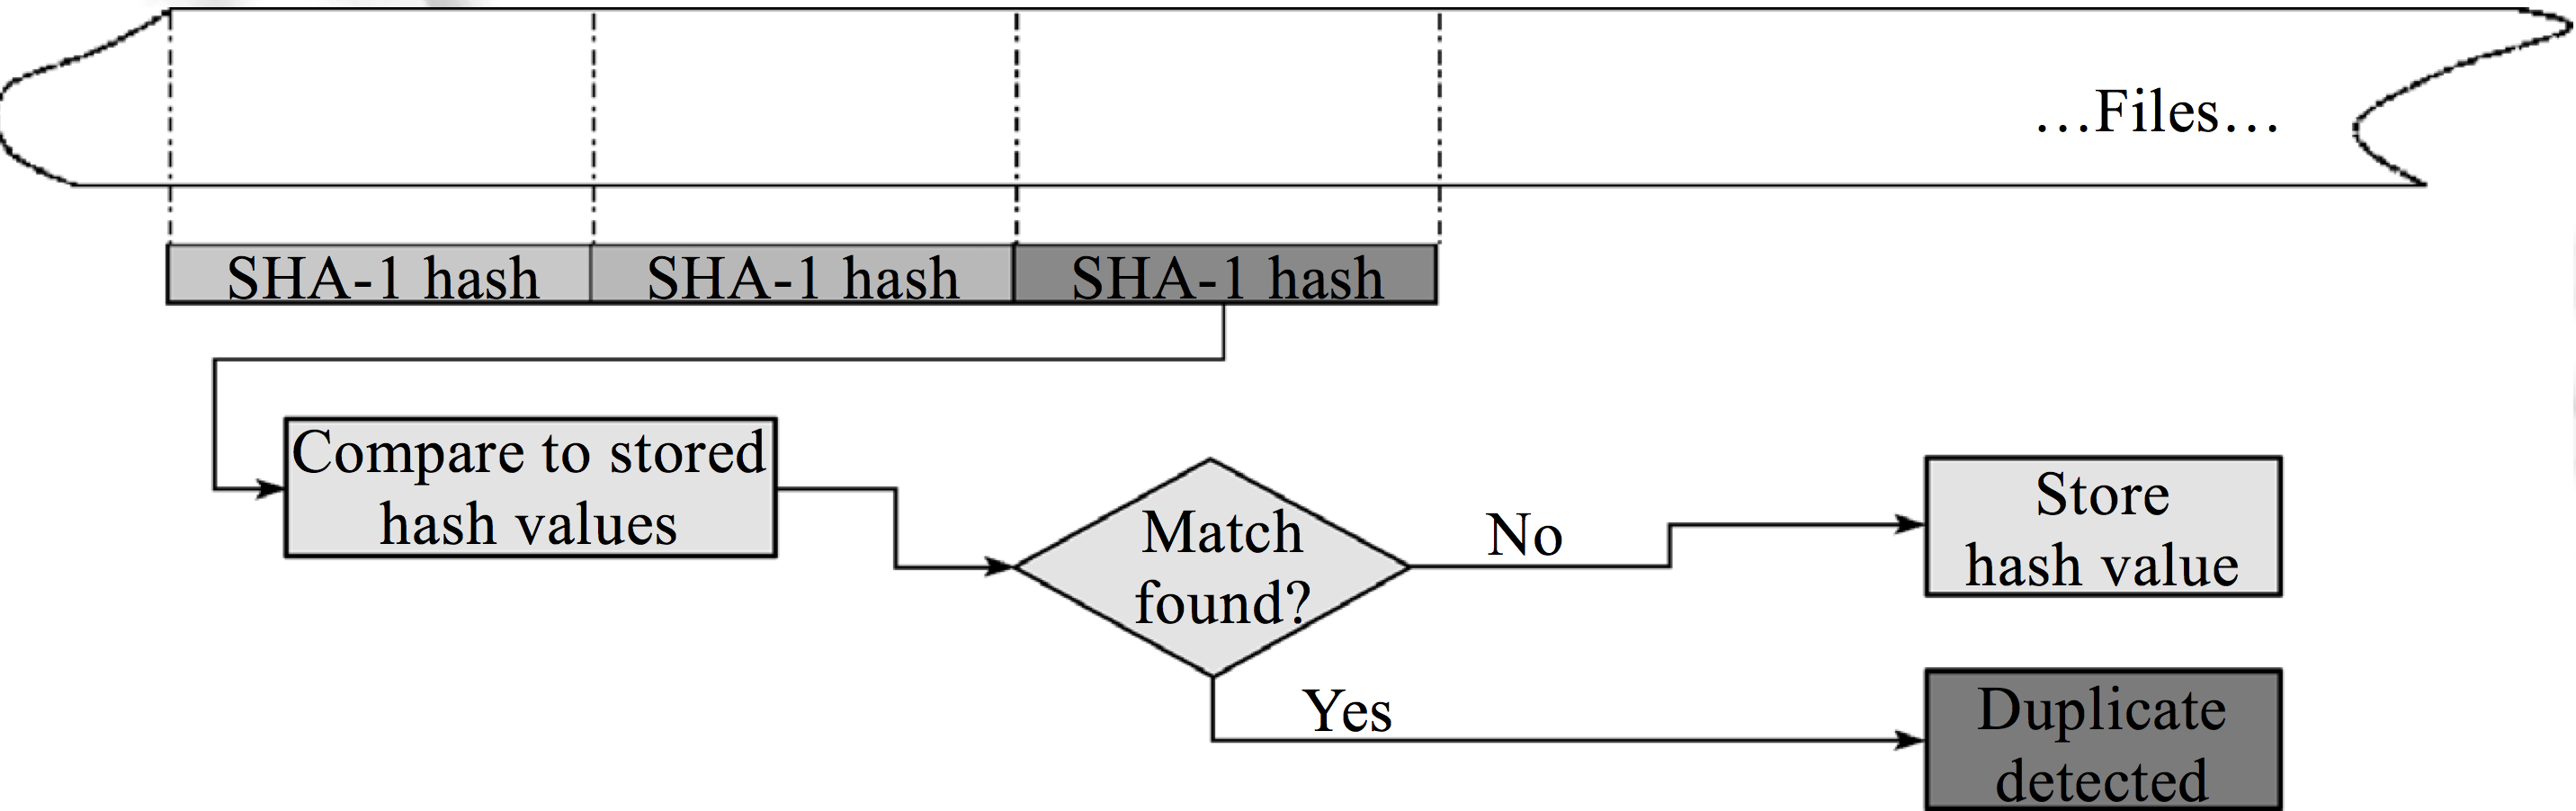
\includegraphics[origin=br,width=15cm]{chap2/fsp.png}
    \bicaption[fig:fsp]{xxx}{FSP技术.}{Fig}{FSP}
    \end{minipage}     
\end{figure}
\section{内容块方法}
\label{sec:contentchunk}

为了解决这个问题,低带宽网络文件系统把文件基于文件内容分成长度可以变化的分块。这个方法的具体做法在图中。

基于文件的内容使用Rabin fingerprints算法将文件分成若干块,原因是这个算法在滑动窗口上计算的效率非常高。一个长度为48字节的滑动窗口被用来来计算每一个重叠48字节文件块的指纹。指纹窗口不断向前移动直到指纹的低字节满足某个预定义的条件,把这个点叫做断点。断点和断点之间的文件块内容被分为一个分块,分块文件的大小由预定义的条件锁定。为了避免一些特殊情况的发生,LBFS建议对分块的长度进行限制。一般来说,取512字节作为最小长度,64K字节作为最大长度。

内容块方法可以很好的解决上面提到的增加字节和删除字节的问题,因为此刻的分块边界是由内容来决定而不是固定长度。一段小数量的字节插入或删除不会影响到一个文件的断点。如果对文件的改变发生在48字节断点区域之外的话,那么边界将不会发生改变,或者如果变化的字节创造了新的断点,那么一个分块可能会变为两个。如果对文件的改变发生在48字节断点区域之内的话,两个文件分块可能合并成一个,即断点被破坏了,或者断点的位置可能会移动,即一个新的断点被引入了,原来的断点被破坏了。最重要的是,无论哪种情况的发生,插入或者删除字节影响的只是一块或者两块文件分块,其余所有分块将不受影响。这个特征使得了内容快方法对只有一小部分不同的文件能够检测出更多的重复数据。

当文件被分块以后,计算每个分块的SHA1哈希值并和之前保存的哈希值比较以检测重复数据。

\begin{figure}[!hbp]
%\centering
    \begin{minipage}[b]{1\textwidth}
    \captionstyle{\centering}
    \centering
    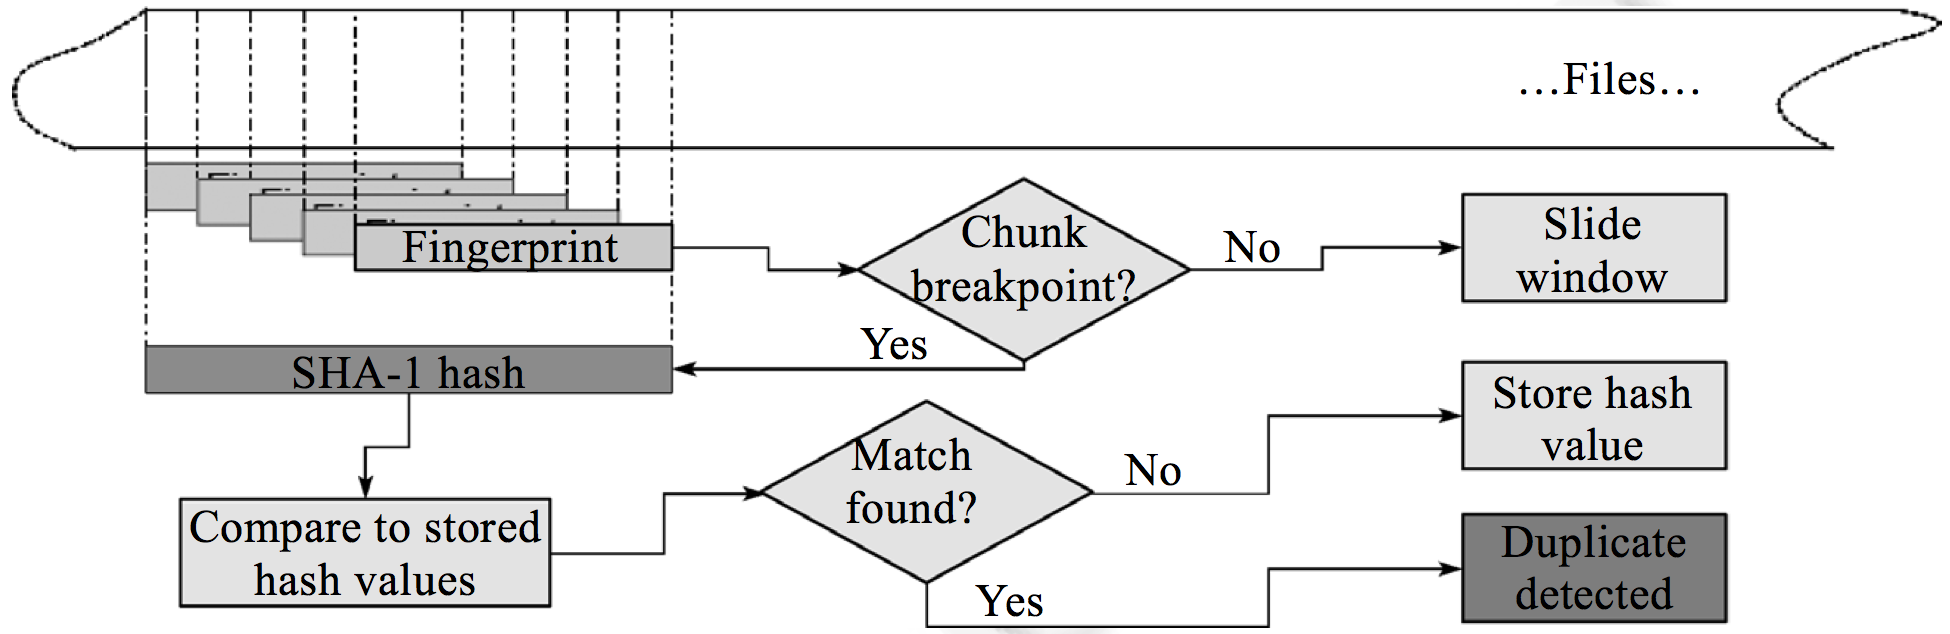
\includegraphics[origin=br,width=15cm]{chap2/ccm.png}
    \bicaption[fig:ccm]{xxx}{CCM技术.}{Fig}{CCM}
    \end{minipage}
\end{figure}

\section{滑动块方法}
\label{sec:slidingblock}

上一节提到的内容块方法解决了插入删除导致边界变化的问题,但引入了新的问题,即长度不同的分块。对于一个存储系统而言,存储固定长度的分块能够降低很大的复杂度和提高效率。在这一节介绍的滑动块方法将结合先前方法的优点并且解决插入问题的同时保持固定长度的分块。图显示了滑动块方法的具体做法。

滑动块方法使用了rsync检验和和一个分块长度的滑动窗口来计算文件中每一个重叠文件段的检验和。rsync检验和算法在滑动窗口上运行速度很快效率很高。每一个文件段的检验和都和以前存储的值相比较。如果发现相同的值,将对文件块更加复杂和消耗计算资源的SHA1算法,和之前存储过的值做比较,如果发现相同,则检测到了重复数据。如果重复被检测到,那么它将被记录下来,然后滑动窗口将移动通过这个块继续工作。另外,在之前的分块的结尾和新检测到重复数据之间的文件段必须被记录和存储。当一个检验和或者哈希值没有被找到,滑动块窗口向前移动,整个过程继续。如果滑动块窗口移动过了整个分块的长度并且没有把它匹配到已有的分块,那么这个分块的检验和和SHA1哈希值将被计算并且存储在它们各自的表中,为了之后的比较。

滑动块方法通过检查每个分块长度的文件块来解决插入问题。如果一小段比特被插入到文件中,只有这个位置周围的分块将发生变化,变化分块的下一块分块将被检测出来,并且被算法所匹配到。相似的,删除一小段比特的文件,变化分块后面的分块将依旧被这个算法检测出来。

\begin{figure}[!hbp]
%\centering
    \begin{minipage}[b]{1\textwidth}
    \captionstyle{\centering}
    \centering
    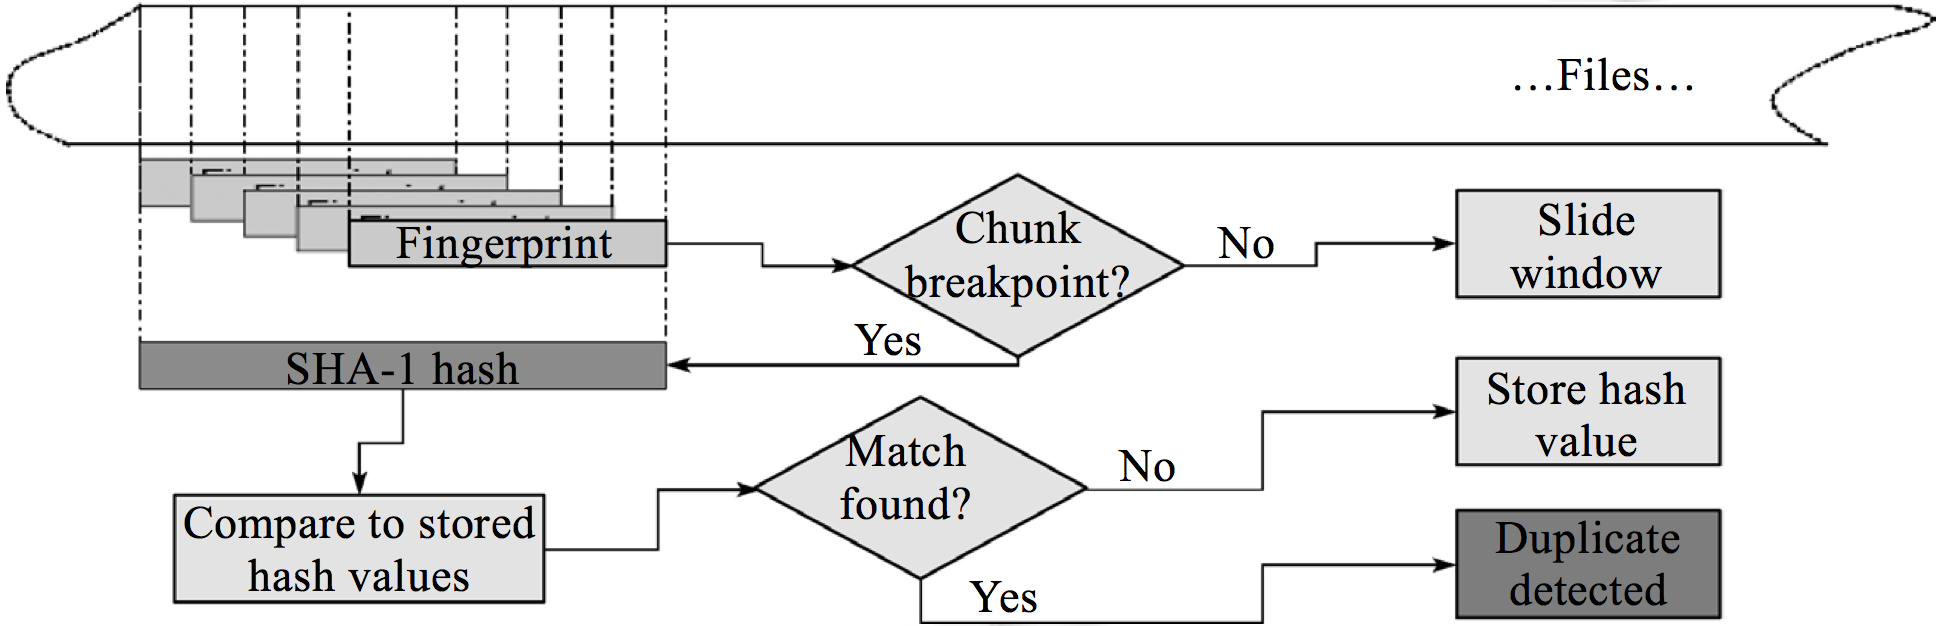
\includegraphics[origin=br,width=15cm]{chap2/sbm.png}
    \bicaption[fig:sbm]{xxx}{SBM技术.}{Fig}{SBM}
    \end{minipage}
\end{figure}

\section{小结}
\label{sec:relatedwork}
本节主要介绍了重复数据检测的四种方法,文献[5]采用了大量的数据集评估了全文件检测、简单分块、内容快方法检测相同数据的效果,并给出了最终实验的对比图。。。。
